\section{Hardware}

\textbf{MPU6050 Sensor:} The MPU6050 is a widely used 6-axis MEMS-based Inertial Measurement Unit (IMU) that integrates a 3-axis accelerometer and a 3-axis gyroscope within a single chip.It is capable of detecting linear acceleration in the range of ±2g to ±16g and angular velocity from ±250°/s to ±2000°/s, making it highly suitable for motion tracking and gesture recognition applications. A notable feature of the MPU6050 is its onboard Digital Motion Processor (DMP), which performs real-time sensor fusion using algorithms such as Kalman or complementary filtering. This significantly reduces noise and drift in gyroscopic data, enabling stable orientation tracking through the calculation of quaternions or Euler angles (roll, pitch, and yaw). The sensor communicates with microcontrollers through the I²C interface, supporting clock speeds between 100 kHz and 400 kHz for efficient data exchange. Its compact design, reliability, and real-time capabilities make it ideal for wearable systems. It enables precise and responsive motion capture for interactive systems in gesture-based applications.

\begin{figure}[htbp!]
\centering
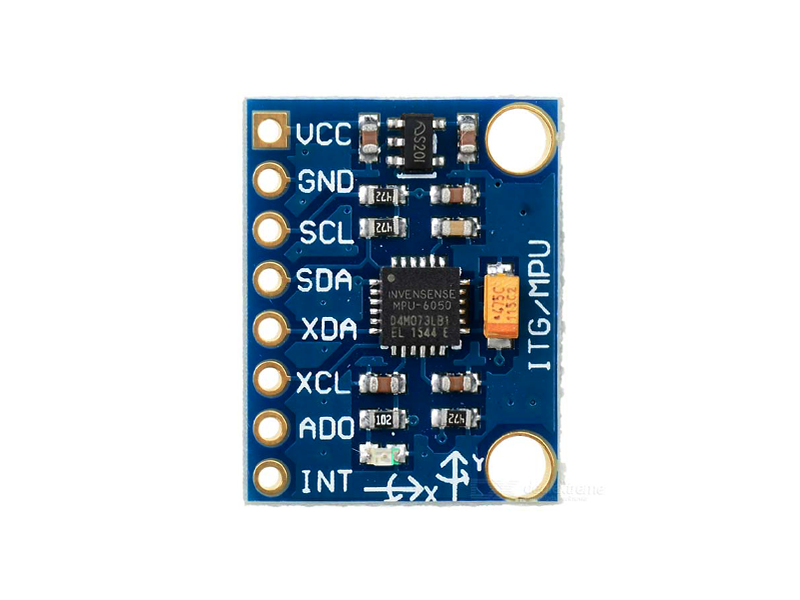
\includegraphics[width=0.5\textwidth]{images/3.1.png}
\caption{\textbf{MPU6050 Sensor}}
\label{fig:3.1}
\end{figure}

\vspace{1.5\baselineskip} % Adds 1.5 line spaces before next section

\textbf{Arduino Mega:} The Arduino Mega is an open-source microcontroller board based on the ATmega2560, designed for projects requiring extensive input/output operations and greater memory capacity. It features 54 digital I/O pins, 16 analog inputs, and four UARTs for serial communication, making it suitable for complex hardware interfacing. With 256 KB of flash memory and a 16 MHz clock speed, it can handle multiple sensors and real-time data processing efficiently. In this project, the Arduino Mega serves as the central controller, managing input from multiple MPU6050 sensors and switches to ensure accurate and synchronized gesture-based interactions within the game environment.

\begin{figure}[htbp!]
\centering
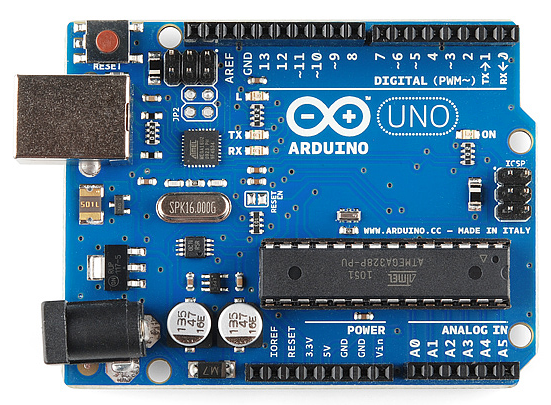
\includegraphics[width=0.5\textwidth]{images/fig3.2.png}
\caption{\textbf{Arduino Uno Board}}
\label{fig:3.2}
\end{figure}

\vspace{1.5\baselineskip} % Adds 1.5 line spaces before next section

\textbf{ESP8266}: The ESP8266 is a low-cost, high-performance Wi-Fi microcontroller based on a 32-bit RISC CPU core (Tensilica L106), operating at 80–160 MHz. It integrates TCP/IP protocol stack and supports IEEE 802.11 b/g/n standards, enabling wireless connectivity with low power consumption (~80 mA active mode). It enables devices to connect to wireless networks and communicate over the internet or within local networks. The ESP8266 supports multiple modes such as station, access point, and both simultaneously, making it highly versatile for wireless communication. It can be programmed using the Arduino IDE and is capable of handling HTTP requests, data transfer, and remote control functionalities. The ESP8266 is used to explore wireless communication possibilities between the hardware controller and the game system, potentially allowing untethered interaction.

\begin{figure}[htbp!]
\centering
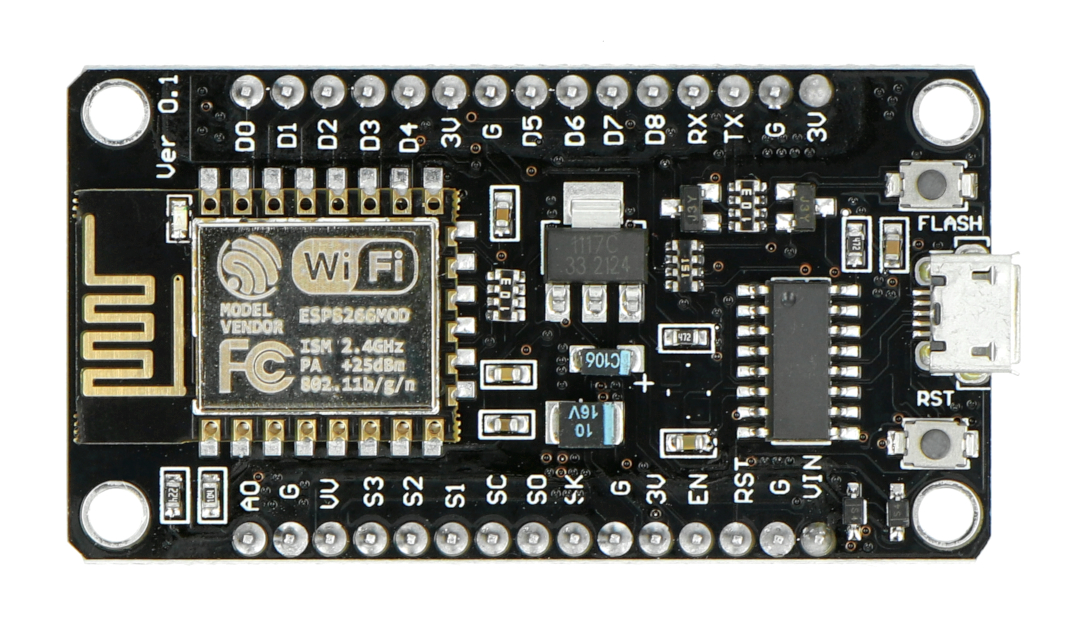
\includegraphics[width=0.5\textwidth]{images/fig3.3.jpg}
\caption{\textbf{ESP8266 Wi-Fi Module}}
\label{fig:3.3}
\end{figure}

\vspace{1.5\baselineskip} % Adds 1.5 line spaces before next section

\textbf{Flex Sensors: }Flex sensors are passive resistive devices that change their resistance based on the amount of bend applied to them. Typically constructed using a flexible substrate coated with conductive ink, their resistance increases as the sensor is bent. This property allows them to detect the degree of bending or curvature, making them suitable for applications involving motion capture, wearable electronics, and gesture recognition. When integrated with microcontrollers, the analog resistance change can be converted into meaningful input data. In this project, flex sensors are considered for detecting finger movements by measuring the degree of bend in each finger.

\begin{figure}[htbp!]
\centering
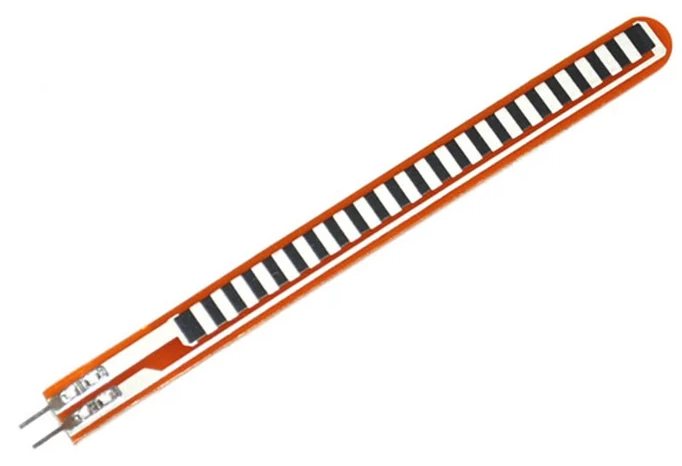
\includegraphics[width=0.5\textwidth]{images/3.4.png}
\caption{\textbf{Flex Sensor}}
\label{fig:3.4}
\end{figure}


\section{Software}
\lipsum[4-8]
%\section{Dataset}
%\lipsum[4-8]
